% Graphic for TeX using PGF
% Title: /home/marcus/Desktop/Diagram1.dia
% Creator: Dia v0.97.3
% CreationDate: Tue Mar 26 09:10:08 2019
% For: marcus
% \usepackage{tikz}
% The following commands are not supported in PSTricks at present
% We define them conditionally, so when they are implemented,
% this pgf file will use them.
\ifx\du\undefined
  \newlength{\du}
\fi
\setlength{\du}{15\unitlength}
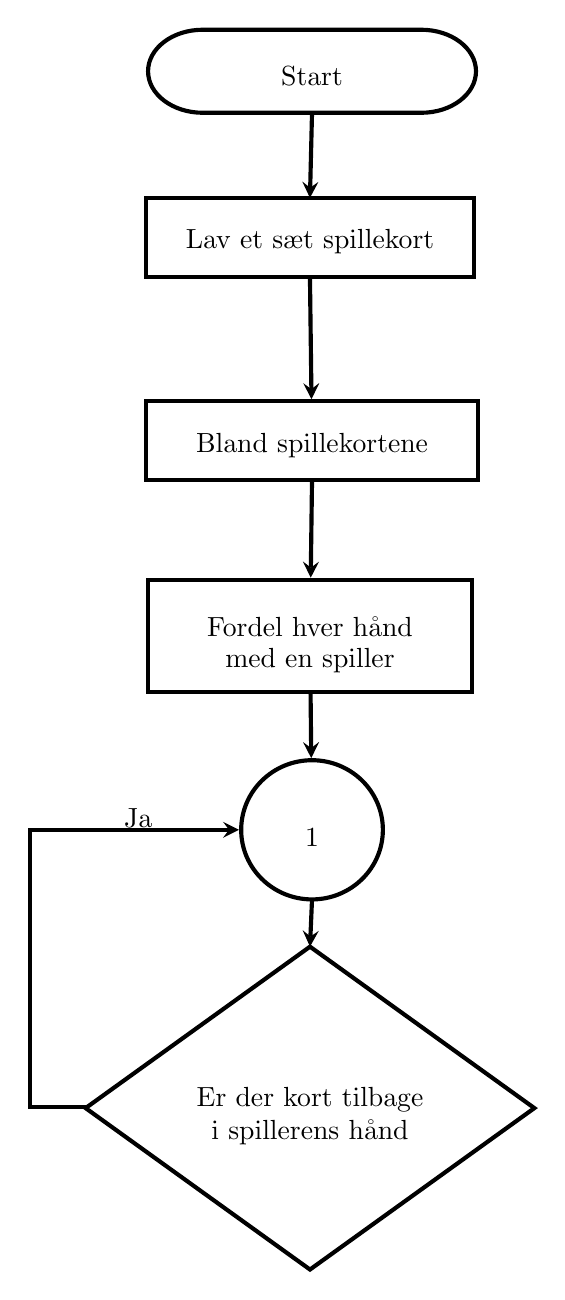
\begin{tikzpicture}
\pgftransformxscale{1.000000}
\pgftransformyscale{-1.000000}
\definecolor{dialinecolor}{rgb}{0.000000, 0.000000, 0.000000}
\pgfsetstrokecolor{dialinecolor}
\definecolor{dialinecolor}{rgb}{1.000000, 1.000000, 1.000000}
\pgfsetfillcolor{dialinecolor}
\pgfsetlinewidth{0.100000\du}
\pgfsetdash{}{0pt}
\pgfsetdash{}{0pt}
\pgfsetbuttcap
\pgfsetmiterjoin
\pgfsetlinewidth{0.100000\du}
\pgfsetbuttcap
\pgfsetmiterjoin
\pgfsetdash{}{0pt}
\definecolor{dialinecolor}{rgb}{1.000000, 1.000000, 1.000000}
\pgfsetfillcolor{dialinecolor}
\pgfpathmoveto{\pgfpoint{4.516667\du}{0.000000\du}}
\pgfpathlineto{\pgfpoint{9.783333\du}{0.000000\du}}
\pgfpathcurveto{\pgfpoint{10.510509\du}{0.000000\du}}{\pgfpoint{11.100000\du}{0.447715\du}}{\pgfpoint{11.100000\du}{1.000000\du}}
\pgfpathcurveto{\pgfpoint{11.100000\du}{1.552285\du}}{\pgfpoint{10.510509\du}{2.000000\du}}{\pgfpoint{9.783333\du}{2.000000\du}}
\pgfpathlineto{\pgfpoint{4.516667\du}{2.000000\du}}
\pgfpathcurveto{\pgfpoint{3.789491\du}{2.000000\du}}{\pgfpoint{3.200000\du}{1.552285\du}}{\pgfpoint{3.200000\du}{1.000000\du}}
\pgfpathcurveto{\pgfpoint{3.200000\du}{0.447715\du}}{\pgfpoint{3.789491\du}{0.000000\du}}{\pgfpoint{4.516667\du}{0.000000\du}}
\pgfusepath{fill}
\definecolor{dialinecolor}{rgb}{0.000000, 0.000000, 0.000000}
\pgfsetstrokecolor{dialinecolor}
\pgfpathmoveto{\pgfpoint{4.516667\du}{0.000000\du}}
\pgfpathlineto{\pgfpoint{9.783333\du}{0.000000\du}}
\pgfpathcurveto{\pgfpoint{10.510509\du}{0.000000\du}}{\pgfpoint{11.100000\du}{0.447715\du}}{\pgfpoint{11.100000\du}{1.000000\du}}
\pgfpathcurveto{\pgfpoint{11.100000\du}{1.552285\du}}{\pgfpoint{10.510509\du}{2.000000\du}}{\pgfpoint{9.783333\du}{2.000000\du}}
\pgfpathlineto{\pgfpoint{4.516667\du}{2.000000\du}}
\pgfpathcurveto{\pgfpoint{3.789491\du}{2.000000\du}}{\pgfpoint{3.200000\du}{1.552285\du}}{\pgfpoint{3.200000\du}{1.000000\du}}
\pgfpathcurveto{\pgfpoint{3.200000\du}{0.447715\du}}{\pgfpoint{3.789491\du}{0.000000\du}}{\pgfpoint{4.516667\du}{0.000000\du}}
\pgfusepath{stroke}
% setfont left to latex
\definecolor{dialinecolor}{rgb}{0.000000, 0.000000, 0.000000}
\pgfsetstrokecolor{dialinecolor}
\node at (7.150000\du,1.120000\du){Start};
\definecolor{dialinecolor}{rgb}{1.000000, 1.000000, 1.000000}
\pgfsetfillcolor{dialinecolor}
\fill (3.150000\du,4.050000\du)--(3.150000\du,5.950000\du)--(11.050000\du,5.950000\du)--(11.050000\du,4.050000\du)--cycle;
\pgfsetlinewidth{0.100000\du}
\pgfsetdash{}{0pt}
\pgfsetdash{}{0pt}
\pgfsetmiterjoin
\definecolor{dialinecolor}{rgb}{0.000000, 0.000000, 0.000000}
\pgfsetstrokecolor{dialinecolor}
\draw (3.150000\du,4.050000\du)--(3.150000\du,5.950000\du)--(11.050000\du,5.950000\du)--(11.050000\du,4.050000\du)--cycle;
% setfont left to latex
\definecolor{dialinecolor}{rgb}{0.000000, 0.000000, 0.000000}
\pgfsetstrokecolor{dialinecolor}
\node at (7.100000\du,5.107500\du){Lav et sæt spillekort};
\definecolor{dialinecolor}{rgb}{1.000000, 1.000000, 1.000000}
\pgfsetfillcolor{dialinecolor}
\fill (3.150000\du,8.950000\du)--(3.150000\du,10.850000\du)--(11.150000\du,10.850000\du)--(11.150000\du,8.950000\du)--cycle;
\pgfsetlinewidth{0.100000\du}
\pgfsetdash{}{0pt}
\pgfsetdash{}{0pt}
\pgfsetmiterjoin
\definecolor{dialinecolor}{rgb}{0.000000, 0.000000, 0.000000}
\pgfsetstrokecolor{dialinecolor}
\draw (3.150000\du,8.950000\du)--(3.150000\du,10.850000\du)--(11.150000\du,10.850000\du)--(11.150000\du,8.950000\du)--cycle;
% setfont left to latex
\definecolor{dialinecolor}{rgb}{0.000000, 0.000000, 0.000000}
\pgfsetstrokecolor{dialinecolor}
\node at (7.150000\du,10.007500\du){Bland spillekortene};
\definecolor{dialinecolor}{rgb}{1.000000, 1.000000, 1.000000}
\pgfsetfillcolor{dialinecolor}
\fill (3.200000\du,13.250000\du)--(3.200000\du,15.950000\du)--(11.000000\du,15.950000\du)--(11.000000\du,13.250000\du)--cycle;
\pgfsetlinewidth{0.100000\du}
\pgfsetdash{}{0pt}
\pgfsetdash{}{0pt}
\pgfsetmiterjoin
\definecolor{dialinecolor}{rgb}{0.000000, 0.000000, 0.000000}
\pgfsetstrokecolor{dialinecolor}
\draw (3.200000\du,13.250000\du)--(3.200000\du,15.950000\du)--(11.000000\du,15.950000\du)--(11.000000\du,13.250000\du)--cycle;
% setfont left to latex
\definecolor{dialinecolor}{rgb}{0.000000, 0.000000, 0.000000}
\pgfsetstrokecolor{dialinecolor}
\node at (7.100000\du,14.395000\du){Fordel hver hånd};
% setfont left to latex
\definecolor{dialinecolor}{rgb}{0.000000, 0.000000, 0.000000}
\pgfsetstrokecolor{dialinecolor}
\node at (7.100000\du,15.195000\du){med en spiller};
\definecolor{dialinecolor}{rgb}{1.000000, 1.000000, 1.000000}
\pgfsetfillcolor{dialinecolor}
\fill (7.101144\du,22.088400\du)--(12.506289\du,25.977221\du)--(7.101144\du,29.866042\du)--(1.696000\du,25.977221\du)--cycle;
\pgfsetlinewidth{0.100000\du}
\pgfsetdash{}{0pt}
\pgfsetdash{}{0pt}
\pgfsetmiterjoin
\definecolor{dialinecolor}{rgb}{0.000000, 0.000000, 0.000000}
\pgfsetstrokecolor{dialinecolor}
\draw (7.101144\du,22.088400\du)--(12.506289\du,25.977221\du)--(7.101144\du,29.866042\du)--(1.696000\du,25.977221\du)--cycle;
% setfont left to latex
\definecolor{dialinecolor}{rgb}{0.000000, 0.000000, 0.000000}
\pgfsetstrokecolor{dialinecolor}
\node at (7.101144\du,25.772221\du){Er der kort tilbage};
% setfont left to latex
\definecolor{dialinecolor}{rgb}{0.000000, 0.000000, 0.000000}
\pgfsetstrokecolor{dialinecolor}
\node at (7.101144\du,26.572221\du){i spillerens hånd};
\pgfsetlinewidth{0.100000\du}
\pgfsetdash{}{0pt}
\pgfsetdash{}{0pt}
\pgfsetmiterjoin
\pgfsetbuttcap
{
\definecolor{dialinecolor}{rgb}{0.000000, 0.000000, 0.000000}
\pgfsetfillcolor{dialinecolor}
% was here!!!
\pgfsetarrowsend{stealth}
{\pgfsetcornersarced{\pgfpoint{0.000000\du}{0.000000\du}}\definecolor{dialinecolor}{rgb}{0.000000, 0.000000, 0.000000}
\pgfsetstrokecolor{dialinecolor}
\draw (1.696000\du,25.977221\du)--(1.696000\du,25.950000\du)--(0.350000\du,25.950000\du)--(0.350000\du,19.273282\du)--(5.393160\du,19.273282\du);
}}
% setfont left to latex
\definecolor{dialinecolor}{rgb}{0.000000, 0.000000, 0.000000}
\pgfsetstrokecolor{dialinecolor}
\node[anchor=west] at (2.350000\du,19.000000\du){Ja};
\definecolor{dialinecolor}{rgb}{1.000000, 1.000000, 1.000000}
\pgfsetfillcolor{dialinecolor}
\pgfpathellipse{\pgfpoint{7.150028\du}{19.273282\du}}{\pgfpoint{1.706728\du}{0\du}}{\pgfpoint{0\du}{1.676682\du}}
\pgfusepath{fill}
\pgfsetlinewidth{0.100000\du}
\pgfsetdash{}{0pt}
\pgfsetdash{}{0pt}
\pgfsetmiterjoin
\definecolor{dialinecolor}{rgb}{0.000000, 0.000000, 0.000000}
\pgfsetstrokecolor{dialinecolor}
\pgfpathellipse{\pgfpoint{7.150028\du}{19.273282\du}}{\pgfpoint{1.706728\du}{0\du}}{\pgfpoint{0\du}{1.676682\du}}
\pgfusepath{stroke}
% setfont left to latex
\definecolor{dialinecolor}{rgb}{0.000000, 0.000000, 0.000000}
\pgfsetstrokecolor{dialinecolor}
\node at (7.150028\du,19.468282\du){1};
\pgfsetlinewidth{0.100000\du}
\pgfsetdash{}{0pt}
\pgfsetdash{}{0pt}
\pgfsetbuttcap
{
\definecolor{dialinecolor}{rgb}{0.000000, 0.000000, 0.000000}
\pgfsetfillcolor{dialinecolor}
% was here!!!
\pgfsetarrowsend{stealth}
\definecolor{dialinecolor}{rgb}{0.000000, 0.000000, 0.000000}
\pgfsetstrokecolor{dialinecolor}
\draw (7.100000\du,5.950000\du)--(7.137347\du,8.900446\du);
}
\pgfsetlinewidth{0.100000\du}
\pgfsetdash{}{0pt}
\pgfsetdash{}{0pt}
\pgfsetbuttcap
{
\definecolor{dialinecolor}{rgb}{0.000000, 0.000000, 0.000000}
\pgfsetfillcolor{dialinecolor}
% was here!!!
\pgfsetarrowsend{stealth}
\definecolor{dialinecolor}{rgb}{0.000000, 0.000000, 0.000000}
\pgfsetstrokecolor{dialinecolor}
\draw (7.150000\du,2.000000\du)--(7.100000\du,4.050000\du);
}
\pgfsetlinewidth{0.100000\du}
\pgfsetdash{}{0pt}
\pgfsetdash{}{0pt}
\pgfsetbuttcap
{
\definecolor{dialinecolor}{rgb}{0.000000, 0.000000, 0.000000}
\pgfsetfillcolor{dialinecolor}
% was here!!!
\pgfsetarrowsend{stealth}
\definecolor{dialinecolor}{rgb}{0.000000, 0.000000, 0.000000}
\pgfsetstrokecolor{dialinecolor}
\draw (7.150000\du,10.850000\du)--(7.118665\du,13.200159\du);
}
\pgfsetlinewidth{0.100000\du}
\pgfsetdash{}{0pt}
\pgfsetdash{}{0pt}
\pgfsetbuttcap
{
\definecolor{dialinecolor}{rgb}{0.000000, 0.000000, 0.000000}
\pgfsetfillcolor{dialinecolor}
% was here!!!
\pgfsetarrowsend{stealth}
\definecolor{dialinecolor}{rgb}{0.000000, 0.000000, 0.000000}
\pgfsetstrokecolor{dialinecolor}
\draw (7.114989\du,16.000216\du)--(7.131548\du,17.547043\du);
}
\pgfsetlinewidth{0.100000\du}
\pgfsetdash{}{0pt}
\pgfsetdash{}{0pt}
\pgfsetbuttcap
{
\definecolor{dialinecolor}{rgb}{0.000000, 0.000000, 0.000000}
\pgfsetfillcolor{dialinecolor}
% was here!!!
\pgfsetarrowsend{stealth}
\definecolor{dialinecolor}{rgb}{0.000000, 0.000000, 0.000000}
\pgfsetstrokecolor{dialinecolor}
\draw (7.150028\du,20.949964\du)--(7.101144\du,22.088400\du);
}
\end{tikzpicture}
